\documentclass{article}
\usepackage[english]{babel}
\usepackage{amsmath}
\usepackage{amssymb}
\usepackage{amsthm}
\usepackage{amsfonts}
\usepackage{blindtext}
\usepackage{systeme}
\usepackage{relsize}
\usepackage{enumerate}
\usepackage{commath}
\usepackage{mathrsfs}
\usepackage{bm}
\usepackage{float}
\usepackage{graphicx}
\usepackage{wrapfig}
\usepackage{subcaption}
\usepackage{tikz-cd}
\usetikzlibrary{automata,positioning}
%\usepackage{hyperref}
%\hypersetup{
% colorlinks=false,% hyperlinks will be black
%linkbordercolor=black,% hyperlink borders will be red
%pdfborderstyle={/S/U/W 0.25}% border style will be underline of width 1pt
%}
\usepackage{chngcntr}
\usepackage{MnSymbol}
\usepackage{tikz}
\usepackage[margin=0.75in]{geometry}
\usepackage{cleveref}

\newcommand{\C}{\mathbf{C}}
\newcommand{\R}{\mathbf{R}}
\newcommand{\Q}{\mathbf{Q}}
\newcommand{\Z}{\mathbf{Z}}
\newcommand{\N}{\mathbf{N}}
\newcommand{\E}{\mathbf{E}}
\newcommand{\B}{\mathbf{B}}
\newcommand{\F}{\mathbf{F}}
\newcommand{\U}{\mathbf{U}}
\newcommand{\V}{\mathbf{V}}
\newcommand{\J}{\mathbf{J}}
\newcommand{\x}{\mathbf{x}}
\newcommand{\y}{\mathbf{y}}
\newcommand{\z}{\mathbf{z}}
\newcommand{\Sb}{\mathbf{S}}
\newcommand{\Cs}{\mathscr{C}}
\newcommand{\As}{\mathscr{A}}
\newcommand{\I}{\textnormal{\textbf{I}}}
\newcommand{\Id}{\dot{\textnormal{\textbf{I}}}}
\newcommand{\Top}{\textnormal{\textbf{Top}}}
\newcommand{\hTop}{\textnormal{\textbf{hTop}}}
\newcommand{\Groups}{\textnormal{\textbf{Groups}}}
\newcommand{\Set}{\textnormal{\textbf{Set}}}
\newcommand{\Xib}{\mathbf{\Xi}}
\newcommand{\Sym}{\text{Sym}}
\newcommand{\prid}[1]{\langle #1 \rangle}
\newcommand{\apoly}[1]{a_{#1} + a_{#1}x+ a_{#1}x^2 + \cdots + a_{#1}x^n}
\newcommand{\dist}{\textnormal{dist}}
\newcommand{\ti}[1]{\textit{#1}}
\newcommand{\tb}[1]{\textnormal{\textbf{#1}}}
\newcommand{\es}{\varnothing}
\newcommand{\sst}{\subset}
\newcommand{\ssteq}{\subseteq}
\newcommand{\func}[3]{#1: #2 \to #3}
\newcommand{\inte}[1]{\textnormal{int}(#1)}
\newcommand{\bdr}[1]{\textnormal{bdry}(#1)}
\newcommand{\ifff}{if and only if }
\newcommand{\st}{such that }
\newcommand{\wrt}{with respect to }
\newcommand{\tspace}[1]{\text{T}_#1}
\newcommand{\mathdash}{\hbox{-}}
\newcommand{\diam}[1]{\textnormal{diam}(#1)}
\newcommand{\setst}{\hspace{1mm} | \hspace{1mm} }
\newcommand{\supp}{\textnormal{support}}
\newcommand{\clos}{\textnormal{closure}}
\newcommand{\rel}{\textnormal{rel }}
\newcommand{\Hom}{\textnormal{Hom}}
\newcommand{\obj}{\textnormal{obj}}
\newcommand{\varlisto}[2]{#1_1,#1_2,\ldots,#1_{#2}}
\newcommand{\varlistz}[2]{#1_0,#1_1,\ldots,#1_{#2}}
\newcommand{\finv}[2]{#1^{-1}(#2)}
\newcommand{\disu}{\rotatebox[origin=c]{90}{$\models$}}
\newcommand{\rank}{\textnormal{rank }}
\newcommand{\card}{\textnormal{card }}
\newcommand{\im}{\textnormal{im }}
\newcommand{\cls}{\textnormal{cls }}
\newcommand{\rev}{\textnormal{rev }}
\newcommand{\defeq}{\mathrel{\stackrel{\makebox[0pt]{\mbox{\normalfont\tiny def}}}{=}}}



%\renewcommand{\phi}{\varphi}
\renewcommand{\epsilon}{\varepsilon}


\newtheorem{theorem}{Theorem}[section]
\newtheorem{corollary}[theorem]{Corollary}
\newtheorem{proposition}{Proposition}[theorem]
\newtheorem{lemma}[theorem]{Lemma}
\theoremstyle{definition}
\newtheorem*{definition}{Definition}
\newtheorem*{remark}{Remark}
\newtheorem*{remarks}{Remarks}


\renewcommand\qedsymbol{$\blacksquare$}
\setcounter{section}{-1}

\counterwithin*{equation}{section}

\title{CSCI 3434 Theory of Computation Homework 2}
\author{Luke Meszar (Worked with Jeff Lipnick)}
\date{September 29, 2017}
\begin{document}
\maketitle
\begin{enumerate}
	\item[HW 3.1] Give regular expressions for each of the following subsets of $\{a,b\}^*$.
	\begin{enumerate}
		\item $\{x \setst x \text{ contains an even numbers of } a\text{'s}\}$
		
		The pattern $((aa)^*b^*+ab^*a)^*$ matches strings with an even number of $a$'s. 
		
		The first part of the Or, $(aa)^*b^*$ will match any string that has an even number of $a$'s followed by any number of $b$'s. Since $(aa)^*$ can match the empty string, it is possible to start a string with a $b$. The second part of the Or, $ab^*a$ will match any string that has two $a$'s separated by any number of $b$'s. The pattern matches either of these two possibilities any number of times. Thus, this patter will match strings \ifff they have an even number of $a$'s.
		
		\item $\{x \setst x \text{ contains an odd numbers of } b\text{'s}\}$
		
		The pattern $(a^*ba^*)((bb)^*a^*+ ba^*b)^*$ matches strings with an odd number of $b$'s.
		
		The first part of the concatenations, $(a^*ba^*)$ guarantees there will always be at least one $b$ which is necessary since every odd number has to form $2k + 1$ for $k \in \Z$. In the second part of the concatenation, we see the same pattern as in part (a) except the $a$'s and $b$'s are reversed. This gives the $2k$ part of the equation for an odd number. Thus, this pattern matches strings \ifff they have an odd number of $b$'s. 
	\end{enumerate}
\item[HW 3.2] Give deterministic finite automata accepting the set of strings matching the following regular expressions.
\begin{enumerate}
	\item $(000^*+111^*)^*$.
	
	We begin by constructing an NFA that accepts $000^*$. 
	
	\begin{center}
		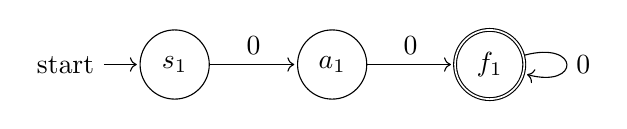
\begin{tikzpicture}[shorten >=1pt,node distance=2cm,on grid,auto]	
		\node[state,initial](s1) {$s_1$};
		\node[state](a1)[right of=s1] {$a_1$};
		\node[state,accepting](f1)[right of=a1] {$f_1$};
		\path[->]
		(s1) edge node {0} (a1)
		(a1) edge node {0} (f1)
		(f1) edge [loop right] node {0} (f1);
		\end{tikzpicture}
	\end{center}
	This NFA accepts strings that have at least 2 00's which is what the pattern $000^*$ matches. 
	
	Likewise, we can construct an NFA that accepts $111^*$. 
	
	\begin{center}
		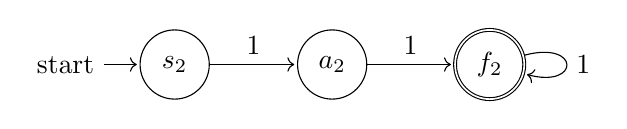
\begin{tikzpicture}[shorten >=1pt,node distance=2cm,on grid,auto]	
		\node[state,initial](s2) {$s_2$};
		\node[state](a2)[right of=s2] {$a_2$};
		\node[state,accepting](f2)[right of=a2] {$f_2$};
		\path[->]
		(s2) edge node {1} (a2)
		(a2) edge node {1} (f2)
		(f2) edge [loop right] node {1} (f2);
		\end{tikzpicture}
	\end{center}

	Then we can combine them into an NFA that accepts $000^* + 111^*$ using $\epsilon$-transitions.
	\begin{center}
		\begin{tikzpicture}[shorten >=1pt,node distance=2cm,on grid,auto]
		\node[state,initial](s) {$s$};
		\node[state](a1)[above right of=s] {$a_1$};
		\node[state,accepting](f1)[right of=a1] {$f_1$};	
		\node[state](a2)[below right of=s2] {$a_2$};
		\node[state,accepting](f2)[right of=a2] {$f_2$};
		\path[->]
		(a2) edge [swap] node {1} (f2)
		(f2) edge [loop right,swap] node {1} (f2)
		(a1) edge node {0} (f1)
		(f1) edge [loop right] node {0} (f1)
		(s) edge node {0} (a1)
		(s) edge [swap] node {1} (a2);
		\end{tikzpicture}
	\end{center}

	Finally, we construct an NFA that accepts $(000^*+111^*)^*$ using $\epsilon$-transitions. 
	\begin{center}
		\begin{tikzpicture}[shorten >=1pt,node distance=2cm,on grid,auto]
		\node[state,initial](s) {$s$};
		\node[state](a1)[above right of=s] {$a_1$};
		\node[state,accepting](f1)[right of=a1] {$f_1$};	
		\node[state](a2)[below right of=s2] {$a_2$};
		\node[state,accepting](f2)[right of=a2] {$f_2$};
		\path[->]
		(a2) edge [swap] node {1} (f2)
		(f2) edge [loop right,swap] node {1} (f2)
		(a1) edge node {0} (f1)
		(f1) edge [loop right] node {0} (f1)
		(s) edge node {0} (a1)
		(s) edge [swap] node {1} (a2)
		(f1) edge node {$\epsilon$} (s)
		(f2) edge [swap] node {$\epsilon$} (s);
		\end{tikzpicture}
	\end{center}


	Next we use $\epsilon$-closures $C_{\epsilon}(A)$ as defined on page 318 of Kozen and the subset construction to construct an equivalent DFA. The $\epsilon$-closures are as follows:
	\begin{align*}
		C_{\epsilon}(s) &= \{s\} \\
		C_{\epsilon}(a_1) &= \{a_1\} \\
		C_{\epsilon}(a_2) &= \{a_2\} \\
		C_{\epsilon}(f_1) &= \{f_1,s\} \\
		C_{\epsilon}(f_2) &= \{f_2,s\} \\
	\end{align*}
	
	Then we use the subset construction to find an equivalent DFA\footnote{Method taken from https://www.youtube.com/watch?v=oEraHUCwFVU}:
	\begin{center}
		\begin{tabular}{cccc}
			& & 0 & 1 \\\cline{3-4}
			$\rightarrow$ & \multicolumn{1}{r|}{$[s]$} &$[a_1]$ & $[a_2]$ \\
			& \multicolumn{1}{r|}{$[a_1]$} & $[f_1]$ & $\es$\\
			& \multicolumn{1}{r|}{$[a_2]$} & $\es$ & $[f_2]$ \\
			& \multicolumn{1}{r|}{F$[f_1]$} & $[f_1,s]$ & $[a_2]$\\
			& \multicolumn{1}{r|}{F$[f_2]$} & $[a_1]$ & $[f_2,s]$\\
			& \multicolumn{1}{r|}{F$[f_1,s]$} & $[f_1,s,a_1]$ & $[a_2]$\\
			& \multicolumn{1}{r|}{F$[f_2,s]$} & $[a_1]$ & $[f_2,s,a_2]$\\
			& \multicolumn{1}{r|}{F$[f_1,s,a_1]$} & $[f_1,s,a_1]$ & $[a_2]$\\
			& \multicolumn{1}{r|}{F$[f_2,s,a_2]$} & $[a_1]$ & $[f_2,s,a_2]$\\
		\end{tabular}
	\end{center}
	
	To avoid the issue of mapping to the empty set in a DFA, we add a new state $Z$ to replace $\es$
		\begin{center}
		\begin{tabular}{cccc}
			& & 0 & 1 \\\cline{3-4}
			$\rightarrow$ & \multicolumn{1}{r|}{$[s]$} &$[a_1]$ & $[a_2]$ \\
			& \multicolumn{1}{r|}{$[a_1]$} & $[f_1]$ & $d$\\
			& \multicolumn{1}{r|}{$[a_2]$} & $d$ & $[f_2]$ \\
			& \multicolumn{1}{r|}{F$[f_1]$} & $[f_1,s]$ & $[a_2]$\\
			& \multicolumn{1}{r|}{F$[f_2]$} & $[a_1]$ & $[f_2,s]$\\
			& \multicolumn{1}{r|}{F$[f_1,s]$} & $[f_1,s,a_1]$ & $[a_2]$\\
			& \multicolumn{1}{r|}{F$[f_2,s]$} & $[a_1]$ & $[f_2,s,a_2]$\\
			& \multicolumn{1}{r|}{F$[f_1,s,a_1]$} & $[f_1,s,a_1]$ & $[a_2]$\\
			& \multicolumn{1}{r|}{F$[f_2,s,a_2]$} & $[a_1]$ & $[f_2,s,a_2]$\\
			& \multicolumn{1}{r|}{$d$} & $d$ & $d$\\
		\end{tabular}
	\end{center}

	Then, using the DFA minimization algorithm, we can make this DFA simpler:
	\begin{table}[H]
		\centering
		
		\label{my-label3}
		\begin{tabular}{llllllllll}
			$[s]$ &         &         &         &         &           &           &               &               &     \\
			& $[a_1]$ &         &         &         &           &           &               &               &     \\
			&         & $[a_2]$ &         &         &           &           &               &               &     \\
			x     & x       & x       & $[f_1]$ &         &           &           &               &               &     \\
			x     & x       & x       &         & $[f_2]$ &           &           &               &               &     \\
			x     & x       & x       &         &         & $[f_1,s]$ &           &               &               &     \\
			x     & x       & x       &         &         &           & $[f_2,s]$ &               &               &     \\
			x     & x       & x       &         &         &           &           & $[f_1,s,a_1]$ &               &     \\
			x     & x       & x       &         &         &           &           &               & $[f_2,s,a_2]$ &     \\
			&         &         & x       & x       & x         & x         & x             & x             & $d$
		\end{tabular}
	\caption{First iteration}
	\end{table}

\begin{table}[H]
	\centering
	\begin{tabular}{llllllllll}
		$[s]$ &         &         &         &         &           &           &               &               &     \\
		x     & $[a_1]$ &         &         &         &           &           &               &               &     \\
		x     & x       & $[a_2]$ &         &         &           &           &               &               &     \\
		x     & x       & x       & $[f_1]$ &         &           &           &               &               &     \\
		x     & x       & x       & x       & $[f_2]$ &           &           &               &               &     \\
		x     & x       & x       &         & x       & $[f_1,s]$ &           &               &               &     \\
		x     & x       & x       & x       &         & x         & $[f_2,s]$ &               &               &     \\
		x     & x       & x       &         & x       &           & x         & $[f_1,s,a_1]$ &               &     \\
		x     & x       & x       & x       &         & x         &           & x             & $[f_2,s,a_2]$ &     \\
		x     & x       & x       & x       & x       & x         & x         & x             & x             & $d$
	\end{tabular}
	\caption{Second iteration}
	\label{my-label}
\end{table}
	From this, we see that $[f_1] \approx [f_1,s] \approx [f_1,s,a_1]$ and $[f_12] \approx [f_2,s] \approx [f_2,s,a_2]$.

Thus, the final DFA's transition table is:
\begin{center}
	\begin{tabular}{cccc}
		& & 0 & 1 \\\cline{3-4}
		$\rightarrow$ & \multicolumn{1}{r|}{$[s]$} &$[a_1]$ & $[a_2]$ \\
		& \multicolumn{1}{r|}{$[a_1]$} & $[F_1]$ & $d$\\
		& \multicolumn{1}{r|}{$[a_2]$} & $d$ & $[F_2]$ \\
		& \multicolumn{1}{r|}{F$[F_1]$} & $[F_1]$ & $[a_2]$\\
		& \multicolumn{1}{r|}{F$[F_2]$} & $[a_1]$ & $[F_2]$\\
		& \multicolumn{1}{r|}{$d$} & $d$ & $d$\\
	\end{tabular}
\end{center}
	
\end{enumerate}
Try to simplify as much as possible. 
\item[ME 15] Give a regular expression equivalent to the following automaton.
\begin{center}
	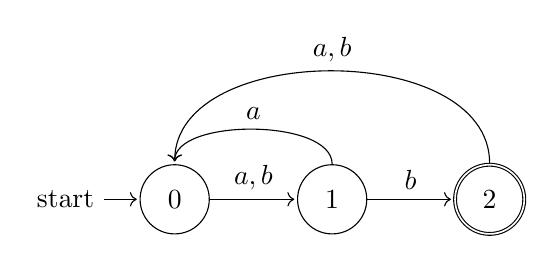
\begin{tikzpicture}[shorten >=1pt,node distance=2cm,on grid,auto]	
	\node[state,initial](s) {$0$};
	\node[state](q1)[right of=s] {$1$};
	\node[state,accepting](q2)[right of=q1] {$2$};
	\path[->]
	(s) edge node {$a,b$} (q1)
	(q1) edge node {$b$} (q2)
	(q1) edge [out=90,in=90,looseness=0.75,swap] node {$a$} (s)
	(q2) edge [out=90,in=90,swap] node {$a,b$} (s);
	\end{tikzpicture}
\end{center}
\begin{align*}\allowdisplaybreaks[1]
&\alpha_{02}^{\{0,1,2\}} = \alpha_{02}^{\{0,2\}}+\alpha_{01}^{\{0,2\}}\left(\alpha_{11}^{\{0,2\}}\right)^*\alpha_{12}^{\{0,2\}} \\
&\text{We begin by expanding the first term} \\
&\alpha_{02}^{\{0,2\}} = \alpha_{02}^{\{0\}} + \alpha_{02}^{\{0\}}\left(\alpha_{22}^{\{0\}}\right)^*\alpha_{22}^{\{0\}} \\
&\alpha_{02}^{\{0\}}  = \alpha_{02}^{\es} + \alpha_{00}^{\es}\left(\alpha_{00}^{\es}\right)^*\alpha_{02}^{\es}\\
&\alpha_{02}^{\es} = \es \\
&\alpha_{00}^{\es} = \epsilon \\
&\alpha_{02}^{\{0\}} = \es + \epsilon\left(\epsilon\right)^*\es = \es \text{ by 9.3 and 9.9} \\
&\alpha_{02}^{\{0,2\}} = \es + \es\left(\alpha_{22}^{\{0\}}\right)^*\alpha_{22}^{\{0\}} = \es + \es = \es \text{ by 9.3 and 9.9} \\
&\text{Next we expand the second term} \\
&\alpha_{01}^{\{0,2\}} = \alpha_{01}^{\{0\}} + \alpha_{02}^{\{0\}}\left(\alpha_{22}^{\{0\}}\right)^*\alpha_{21}^{\{0\}} \\
&\alpha_{01}^{\{0\}} = \alpha_{01}^{\es}+\alpha_{00}^{\es}\left(\alpha_{00}^{\es}\right)^*\alpha_{01}^{\es} \\
&\alpha_{01}^{\es} = a + b \\
&\alpha_{01}^{\{0\}} = \left(a+b\right)+\es\left(\es\right)^*\left(a+b\right)= a + b \\
&\alpha_{01}^{\{0,2\}} = \left(a+b\right) + \es\left(\alpha_{22}^{\{0\}}\right)^*\alpha_{21}^{\{0\}} = a + b\\
&\text{Then we expand the third term} \\
&\alpha_{11}^{\{0,2\}} = \alpha_{11}^{\{2\}}+\alpha_{10}^{\{2\}}\left(\alpha_{00}^{\{2\}}\right)^*\alpha_{01}^{\{2\}} \\
&\alpha_{11}^{\{2\}} = \alpha_{11}^{\es} + \alpha_{12}^{\es}\left(\alpha_{22}^{\es}\right)^*\alpha_{21}^{\es}\\
&\alpha_{11}^{\es} = \epsilon\\
&\alpha_{12}^{\es} = b \\
&\alpha_{22}^{\es} = \epsilon \\
&\alpha_{21}^{\es} = \es \\
&\alpha_{11}^{\{2\}} = \epsilon + b\left(\epsilon\right)^*\es = \epsilon\\
&\alpha_{10}^{\{2\}} = \alpha_{10}^{\es} + \alpha_{12}^{\es}\left(\alpha_{22}^{\es}\right)^*\alpha_{20}^{\es}\\
&\alpha_{10}^{\es} = a \\
&\alpha_{20}^{\es} = a + b \\
&\alpha_{10}^{\{2\}} = a + b\left(\epsilon\right)^*a+b = a + b(a+b) \\
&\alpha_{00}^{\{2\}} =  \alpha_{00}^{\es} + \alpha_{02}^{\es}\left(\alpha_{22}^{\es}\right)^*\alpha_{20}^{\es}\\
&\alpha_{00}^{\{2\}} = \epsilon + \es\left(\epsilon\right)^*(a+b) = \epsilon\\
&\alpha_{01}^{\{2\}}= \alpha_{01}^{\es} + \alpha_{02}^{\es}\left(\alpha_{22}^{\es}\right)^*\alpha_{21}^{\es}\\
&\alpha_{01}^{\{2\}} = a + b + \es\left(\epsilon\right)^*\es = a + b\\
&\alpha_{11}^{\{0,2\}} = \epsilon + (a+b(a+b))(\epsilon)^*(a+b) = \epsilon + (a+b(a+b))(a+b) \\
&\text{Finally we expand the fourth term} \\
&\alpha_{12}^{\{0,2\}} = \alpha_{12}^{\{2\}}+\alpha_{10}^{\{2\}}\left(\alpha_{00}^{\{2\}}\right)^*\alpha_{02}^{\{2\}} \\
&\alpha_{12}^{\{2\}} = \alpha_{12}^{\es} + \alpha_{12}^{\es}\left(\alpha_{22}^{\es}\right)^*\alpha_{22}^{\es}\\ 
&\alpha_{12}^{\{2\}} = b + b(\epsilon)^*\epsilon = b + b = b\\
&\alpha_{02}^{\{2\}} = \alpha_{02}^{\es} + \alpha_{02}^{\es}\left(\alpha_{22}^{\es}\right)^*\alpha_{22}^{\es}\\ 
&\alpha_{02}^{\{2\}} = \es + \es(\epsilon)^*\epsilon = \es \\
&\alpha_{12}^{\{0,2\}} = b + (a+b(a+b))(\epsilon)^*\es = b\\\displaybreak
&\text{Combining all four terms together, we get}\\
&\alpha_{02}^{\{0,1,2\}} = \es + (a+b)(\epsilon + (a+b(a+b))(a+b))^*b \\
&= (a+b)(\epsilon + (a+b(a+b))(a+b))^*b \\
\end{align*}
\begin{align*}
1
\end{align*}
\item[HW 4.1] Show the following sets are not regular.
\begin{enumerate}
	\setcounter{enumii}{1}
	\item $A = \{x \in \{a,b,c\}^* \setst x \text{ is a palindrome; i.e.,} x = \rev x\}$. (use the pumping lemma thoroughly)
	Let $k \geq 0$. Choose $x = \epsilon$, $y = a^k$ and $z = bcb(a)^k$. This is a palindrome since there are an equal number of $a$ on the left and right sides of the string and the $bcb$ in the middle is a palindrome. We can also see that $|y| \geq k$ since $|y| = k$. Now, for all $uvw$ such that $y = uvw$ and $v \neq \epsilon$ we will show there exists an $i \geq 0$ such that $uv^iw \not\in A$. Any $uvw$ can be written as $a^pa^qa^r$ where $p + q + r = k$ and $q > 0$. Then, choose $i \geq 2$. Then $uv^iw = a^pa^{iq}a^r$. Thus $|uv^iw| =p+iq+r > k$. This means that $xuv^iwz$ is of the form $a^lbcba^k$ where $l > k$. This string is no longer a palindrome since there are more $a$s on the left than on the right so the reverse string will not be the same. Thus, palindromes are not regular languages. 
	\setcounter{enumii}{3}
	\item The set PAREN of balanced parentheses ( ). For example, the string ( ( ( ) ( ) ) ( ) ) is in PAREN, but the string ) ( () is not.
	
	For $k > 0$, let $x = (^k, y = )^k,$ and $z = \epsilon$. This string is in PAREN since the number of opening parenthesis is the same as the number of closing parenthesis. We can also see that $|y| \geq k$ since $|y| = k$. Then, for all $uvw = y$ such that $|v| > 0$, we know that $v = )^m$ where $m \leq k$. Write $uvw$ as $)^l)^m)^n$ where $l+m+n = k$ and $m > 0$. Then, choose $i \geq 2$. Thus, $uv^iw = )^l[)^m]^i)^n = )^l)^im)^n$. Thus $|uv^iw| = l + im + n > k$. This means that there are now more closing parenthesis in $uv^iw$ than opening parenthesis in $x$ so $xuv^iwz \not\in$ PAREN.
\end{enumerate}
\item[ME 37] Which of the following sets are regular and which are not? Give justification.
\begin{enumerate}
	\item $A = \{a^nb^{2m} \setst n \geq 0 \text{ and } m \geq 0\}$
	
	Assume that $A$ is regular. Then $\rev A$ is also regular. Define $\func{h}{\{a,b\}^*}{\{a,b\}^*}$ by $h(a) = b$ and $h(b) = a$. Then, consider $A' = h(\rev A)$. This language should also be regular since $h$ is a homomorphism. Finally, the language $A \cap A'$ should also be regular. There are two cases to consider with this intersection. If $n < 2m$, then 
	\[A \cap A' = \{a^nb^n \setst n \geq 0\}\]\
	which we know is not regular. 
	
	If, $n > 2m$, then 
	\[A \cap A' = \{a^{2m}b^{2m} \setst m \geq 0\}.\]
	
	The set $\{a^{2m}b^{2m} \setst m \geq 0\}$ can be easily be seen to be non regular via the pumping lemma. For $k \geq 0$, let $x = a^2k, y = b^2k,$ and $z = \epsilon$. Then for any $u,v,w$ such that $uvw = y$, choose $i \geq 2$. Then $|uv^iw| \geq 2k$ so $xuv^iwz \not \in \{a^{2m}b^{2m} \setst m \geq 0\}$. 
	
	Since $A \cap A'$ is not regular, than our assumption that $A$ is regular must be wrong. Therefore, $A$ is not regular. 
	
	\item $B = \{a^nb^m \setst n = 2m\} $
	
	This is the same as the set $\{a^{2m}b^m \setst m \geq 0\}$. Then, let $x = \epsilon, y = a^{2k},$ and $z = b^k$. This string is clearly in $B$ and $|y| = 2k$. Then, choose $i \geq 2$. Thus $|uv^iw| > 2k$ so $xuv^iwz \not\in B$ since it is not of the form $a^{2m}b^{m}$. Thus, $B$ is not regular. 
	\item $C = \{a^nb^m \setst n \neq m\}$
	
	Assume that $C$ is regular. Then $\sim C$ is also regular. Now, take the following intersection
	\[\sim C \cap L(a^*b^*)\]
	We know that $L(a^*b^*)$ is regular since it is the language of a valid regular expression. The result of this intersection is $\{a^nb^n \setst n \geq 0\}$. To see that this is the result of the intersection, we note that $L(a^*b^*)$ are any string of the form, some number $a$'s followed by some number of $b$'s. If the number of $a$'s and $b$'s were different, it would mean this string would not be in $\sim C$. Thus, the strings have to have the same number of $a$'s and $b$'s. Since $\{a^nb^n \setst n \geq 0\}$ is not regular, then $C$ cannot be regular either. 
	\item $D = \{a^{p-1} \setst p \text{ is prime}\}$
	
	If $D$ where regular, then $\{a\}D$ should be regular due to regular languages being closed under concatenation. However, $\{a\}D = \{aa^{p-1} \setst p \text{ is prime}\}$ = $\{a^p \setst  p \text{ is prime}\}$. But, we know that this set is not regular. 
	
	\item $E = \{xcx \setst x \in \{a,b\}^*\}$
	
	Given $k \geq 0$, consider $x = \epsilon, y = a^k$ and $z = ca^k$. Then $xyz \in E$ since $a^k \in \{a,b\}^*$ and thus $xyz$ has the form $xcx$ and we can see that $|y| = k$. Let $uvw$ be such that $y = uvw$ and $v \neq \epsilon$. Let $i \geq 2$. Then $|uv^iw| > k$ (same logic as 4.1b). This means that $xuv^iwz = a^lca^k$ where $l > k$ so which means this string is not of the form $xcx$. Thus, $E$ is not regular. 
	\item $F =\{xcy \setst x,y \in \{a,b\}^*\}$
	
	Consider the following $DFA$:
	\begin{center}
		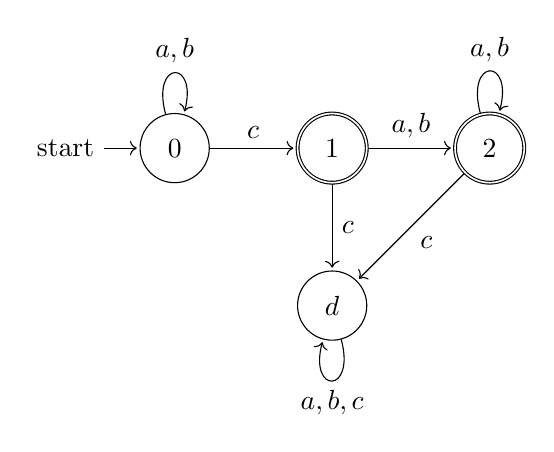
\begin{tikzpicture}[shorten >=1pt,node distance=2cm,on grid,auto]	
		\node[state,initial](s) {0};
		\node[state,accepting](q1)[right of=s] {1};
		\node[state,accepting](q2)[right of=q1] {2};
		\node[state](d)[below of=q1] {$d$};
		\path[->]
		(s) edge node {$c$} (q1)
		(q1) edge node {$a,b$} (q2)
		(s) edge [loop above] node {$a,b$} (s)
		(q2) edge [loop above] node {$a,b$} (q2)
		(q1) edge node {$c$} (d)
		(q2) edge node {$c$} (d)
		(d) edge [loop below] node {$a,b,c$} (d);
		\end{tikzpicture}
	\end{center}
	This DFA works by either accepting as soon as it has seen one has seen one $c$ so strings of the form $xc\epsilon$ are accepted or accepting if any more $a$'s or $b$'s are seen. However, if another $c$ is seen, then it fails to accept. Thus, $F$ is regular. 
	\item $G = \{a^nb^{n+481} \setst n \geq 0 \}$
	
	Given $k \geq 0$, then let $x = a^k, y = b^{k+481}$, and $z = \epsilon$. We have $xyz \in G$ and $|y| > k$. For all $uvw = y$, let $i \geq 2$. Then $|uv^iw| > k + 481$, say $l + 481$. Then $xuv^iwz \not\in G$ because it is not of the form $a^nb^{n+481}$ since $l \neq k$. Thus $G$ is not regular. 
	\item $H = \{a^nb^m \setst n-m \leq 481\}$
	
	Given $k \geq 0$, let $x = \epsilon, y = a^k, z = b^k$. Then $xyz \in H$ since $k - k = 0 \leq 481$. Now for any $u,v,w$ such that $y=uvw$ and $v \neq \epsilon$, then choose $i \geq 482$. The smallest $v$ can be is if it just the symbol $a$. In this case, $|uv^iw| = k + 482$. Thus, $n - m = k + 481 - k = 482 \not\leq 481$. For any other choice of $v$, we will have $|uv^iw| > k + 482$ so it will still fail. Thus $xuv^iwz \not\in H$ and so $H$ is not regular. 
	\item $I = \{a^nb^m\setst n \geq m \text{ and } m \leq 481\}$
	
	This language is regular. Consider the language $I' = \{a^nb^m\setst n \geq m \text{ and } m \leq 2\}$. This is essentially the same language as $I$ since it just differs by a constant. We will only have to change the DFA necessary to accept $I$ by a finite number of states. The following DFA accepts $I'$:
	\begin{center}
		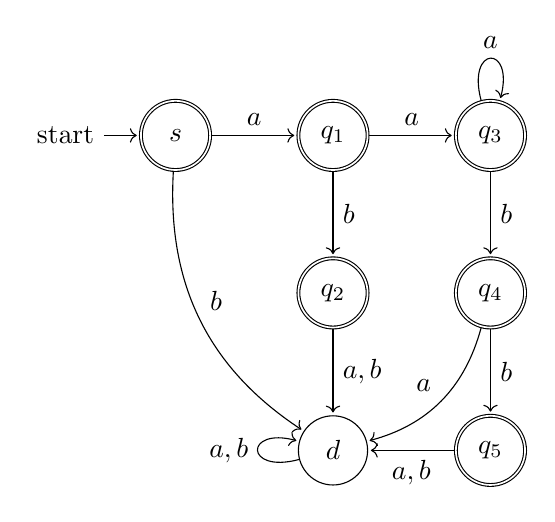
\begin{tikzpicture}[shorten >=1pt,node distance=2cm,on grid,auto]	
		\node[state,initial,accepting](s) {$s$};
		\node[state,accepting](q1)[right of=s] {$q_1$};
		\node[state,accepting](q2)[below of=q1] {$q_2$};
		\node[state,accepting](q3)[right of=q1] {$q_3$};
		\node[state,accepting](q4)[below of=q3] {$q_4$};
		\node[state,accepting](q5)[below of=q4] {$q_5$};
		\node[state](d)[below of=q2] {$d$};
		\path[->]
		(s) edge node {$a$} (q1)
		(q1) edge node {$a$} (q3)
		(q3) edge [loop above] node {$a$} (q3)
		(q1) edge node {$b$} (q2)
		(q2) edge node {$a,b$} (d)
		(d) edge [loop left] node {$a,b$} (d)
		(q3) edge node {$b$} (q4)
		(q4) edge node {$b$} (q5)
		(q5) edge node {$a,b$} (d)
		(q4) edge [bend left,swap] node {$a$} (d)
		(s) edge [bend right] node {$b$} (d);
		\end{tikzpicture}
	\end{center}
	We can see that this DFA does accept $I'$ by considering a few different cases. First, it accepts $\epsilon$. Next, if there is only one $a$, then there can only be one $b$ as denoted by the path from state $q_1$ to $q_2$. If there are 2 or more $a$'s in the string, then we can accept up to the maximum number of $b$'s which is two. This can be seen by the path $q_1$ to $q_3$ to $q_4$ to (potentially) $q_5$. We can also accept any number of $a$'s followed by no $b$'s. If we see too many $b$'s or we see an $a$ after a $b$ we go to the state $d$. If we see a $b$ before any $a$'s, then we also go to $d$. 
	
	A machine of this form can be extended to actually accept $I$. Thus, $I$ is regular. 
	\item $J = \{a^nb^m\setst n \geq m \text{ and } m \geq 481\}$ 
	
	Given $k \geq 0$, let $z = a^l, y = b^l$ and $z = \epsilon$ such  that $l \geq k$ and $l \geq 481$. Then, $xyz \in J$ since $n = l = m \geq 481$. Then for all $u,v,w$ such that $y = uvw$ and $v \neq \epsilon$, choose $i \geq 2$. Then $|uv^iw| > l$. This means that $xuv^iwz \not\in J$ since it is no longer true that $n \geq m$.  
	
	\item $K = L((a^*b)^*a^*)$  	
	
	The pattern $(a^*b)^*a^*$ is a valid regular expression which means that it is a regular language. 
	\item $L = \{a^nb^nc^n \setst n \geq 0\}$
	
	Given $k \geq 0$, let $x = a^k, y = b^k$ and $z = c^k$. Then for all $u,v,w$ such that $y = uvw$ and $v \neq \epsilon$, choose $i \geq 2$. Then $|uv^iw| > k$ so $xuv^iwz \not\in L$ since not all of the exponents are the same anymore. Thus, $L$ is not regular. 
	\item $M$ \{syntactically correct Python programs\}
	
	This language is not regular. An example of a syntatically correct Python program is
	\begin{verbatim}
	arr = ['a','a',...,'a'] //where there are p a's, p prime
	\end{verbatim}
	This is essentially the language $A = \{a^p \setst p \text{ prime}\}$. In fact, it is the language 
	\[A = \{\text{arr} = [('a',)^p] \setst p \text{ prime}\}.\]
	There are simple DFAs that can accept arr = [ ] since it is just a constant string. However, accepting $\{('a',)^p \setst p \text{ prime}\}$ is impossible since this language is isomorphic to $\{a^p \setst p \text{ prime}\}$.
\end{enumerate}
\item[HW 4.3] For the following automata
\begin{center}
	\begin{tabular}{cccc}
		& & a & b \\\cline{3-4}
		$\rightarrow$ & \multicolumn{1}{c|}{1} &1 & 4\\
		& \multicolumn{1}{c|}{2} & 3 & 1\\
		& \multicolumn{1}{c|}{3F} & 4 & 2\\
		& \multicolumn{1}{c|}{4F} & 3 & 5\\
		& \multicolumn{1}{c|}{5} & 4 & 6\\
		& \multicolumn{1}{c|}{6} & 6 & 3\\
		& \multicolumn{1}{c|}{7} & 2 & 4\\
		& \multicolumn{1}{c|}{8} & 3 & 1\\
	\end{tabular}
\end{center}
\begin{enumerate}
	\item say which states are accessible and which are not;
	
	The inaccessible states are 7 and 8. The DFA with only accessible states is as follows:
	\begin{center}
		\begin{tabular}{cccc}
			& & a & b \\\cline{3-4}
			$\rightarrow$ & \multicolumn{1}{c|}{1} &1 & 4\\
			& \multicolumn{1}{c|}{2} & 3 & 1\\
			& \multicolumn{1}{c|}{3F} & 4 & 2\\
			& \multicolumn{1}{c|}{4F} & 3 & 5\\
			& \multicolumn{1}{c|}{5} & 4 & 6\\
			& \multicolumn{1}{c|}{6} & 6 & 3.\\
		\end{tabular}
	\end{center}
	\item list the equivalence classes of the collapsing relation $\approx$ defined in Lecture 13:
	
	\[p \approx q  \overset{\text{def}}{\iff}\forall x \in \Sigma^*, (\hat{\delta}(p,x) \in F \iff \hat{\delta}(q,x)\in F);\]
	
	We begin by marking pairs of states, $\{p,q\}$ if $p \in F$ and $q \not\in F$ or vice versa.
	\begin{table}[H]
		\centering
		\caption{}
		\label{my-label}
		\begin{tabular}{llllll}
			1 &   &   &   &   &   \\
			x & 2 &   &   &   &   \\
			x & x & 3 &   &   &   \\
			x & x &   & 4 &   &   \\
			&   & x & x & 5 &   \\
			&   & x & x &   & 6
		\end{tabular}
	\end{table}
	
	After going through the states again and marking states if $\{\delta(p,a),\delta(q,a)\}$ is already marked, we get.
	\begin{table}[H]
		\centering
		\caption{}
		\label{my-label2}
		\begin{tabular}{llllll}
			1 &   &   &   &   &   \\
			x & 2 &   &   &   &   \\
			x & x & 3 &   &   &   \\
			x & x &   & 4 &   &   \\
			x &   & x & x & 5 &   \\
			& x & x & x & x & 6
		\end{tabular}
	\end{table}
Recursing further will not change anything. Thus, the equivalent states are
\begin{gather*}
1 \approx 6 \\
2 \approx 5 \\
3 \approx 4. \\
\end{gather*}
Denote $1 \approx 6$ as $p$, $2 \approx 5$ as $q$ and $3 \approx 4$ as $r$. 
	\item give the automaton obtained by collapsing equivalent states and removing inaccessible states.
	The automaton with obtained by collapsing equivalent states and removing inaccessible states is:
	
		\begin{center}
			\begin{tabular}{cccc}
				& & a & b \\\cline{3-4}
				$\rightarrow$ & \multicolumn{1}{c|}{$p$} &$p$ & $r$\\
				& \multicolumn{1}{c|}{$q$} & $r$ & $p$\\
				& \multicolumn{1}{c|}{$r$F} & $r$ & $q$\\
			\end{tabular}
		\end{center}
\end{enumerate}
%\item[HW 3.3](Extra Credit) For any set of strings $A$, define the set
%\[\text{MiddleThirds } A = \{y\setst \exists x,z |x| = |y| = |z| \text{ and } xyz \in A\}\]
%For example, MiddleThirds$\{\epsilon,a,ab,bab,bbab,aabbab\} = \{\epsilon,a,bb\}$. Show that if $A$ is regular, then so is MiddleThirds $A$.
\end{enumerate}
\end{document}